\documentclass{article}
\usepackage[a4paper, total={6in, 8in}, margin=20mm]{geometry}
\usepackage{graphicx}
\usepackage{hyperref}
\parindent=0pt
\parskip=12pt

\begin{document}
	The OPTIMADE API enables a user to obtain material information from multiple providers with the same filter query. This is particularly useful when applying machine learning techniques on the obtained materials data. Being able to query multiple providers using a single API allows one to combine data from multiple sources, which may have different ``strengths''.
	
	The OPTIMADE API is used to get materials satisfying the filter query 
	
	\begin{quote}
		`elements HAS ANY ``W",``Al",``Cd",``Zn" AND NOT elements HAS ANY ``B", ``Cl", ``F", ``H", ``N", ``O", ``S", ``Se" AND nelements$>$=5'		
	\end{quote}
	
	from three different providers (anonymized as P1, P2, P3). The number of materials returned by each provider is show in \autoref{fig: exampleFig}(a). A Venn diagram (\autoref{fig: exampleFig}) of the sets of unique elements that appear in the materials from each provider shows that each provider returns a different set of materials for the same filter query.
	
	
	
	A Random Forest Regressor trained on data from all the providers performs much better (R$^2 = 0.98$) 
	
	OPTIMADE simplifies the workflow in many different machine learning applications. 
	\begin{figure}[h]
		\centering
		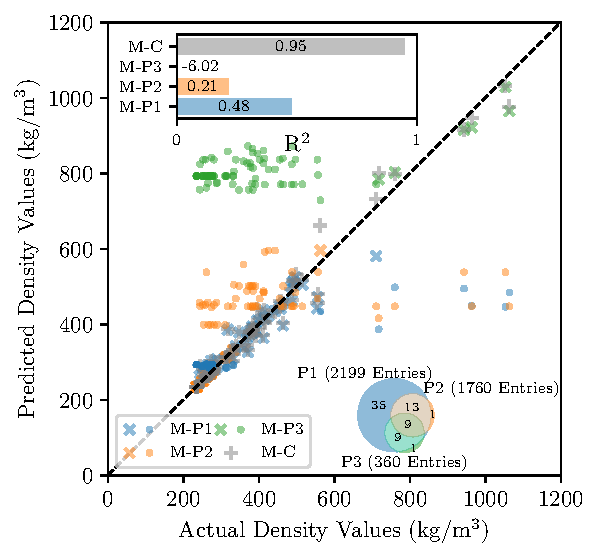
\includegraphics[]{scatterPlot.pdf}
		\caption{Predicted versus actual density} 
		\label{fig: exampleFig}
	\end{figure}
\end{document}